% Copyright 2007 by Till Tantau
%
% This file may be distributed and/or modified
%
% 1. under the LaTeX Project Public License and/or
% 2. under the GNU Public License.
%
% See the file doc/licenses/LICENSE for more details.


\lecture[21]{The $F$ test}{lecture-text}

\subtitle{and two-way ANOVA}

\date{16 November 2015}

% 427-436, 449-456

\begin{document}

\begin{frame}
  \maketitle
\end{frame}



\begin{frame}{Last time}
  \begin{itemize}
    \item \structure{Goal:} test for homogeneity in means among multiple ($>2$) groups of independent samples.
    \item \structure{Tool:} comparison of 
      \item how much variation there is within groups \\
        (around the group means)
      \item and how much variation there is between group means;
      \item quantified by the decomposition of the total sum-of-squares into ``within'' and ``between'' components.
          \[ 
       \SS(\text{total})  = \SS(\text{within}) + \SS(\text{between})  
   \]
  \end{itemize}

  Equations:
    \begin{align*}
        \SS(\text{total}) &= \sum_{ij} (y_{ij} - \bar {\bar y} )^2 
    &  \df(\text{total}) &= n_\cdot - 1 \\
      \SS(\text{within}) &= \sum_{i} (n_i-1) s_i^2 = \sum_{ij} (y_{ij}-\bar y_i)^2 
   &   \df(\text{within}) &= n_\cdot - I \\
      \SS(\text{between}) &= \sum_{i} n_i (\bar y_i - \bar{\bar y})^2 
      & \df(\text{between}) &= I - 1 \\
    \end{align*}
    and the ``mean square'' is $\MS = \SS / \df$.
    
\end{frame}


%%%%%%
\begin{frame}{Example}

    Weight gain of lambs on three diets:
    \begin{center}
        \begin{tabular}{cccc}
            & Diet 1 & Diet 2 & Diet 3 \\
            \hline
            & 8 & 9 & 15 \\
            & 16 & 16 & 10 \\
            & 9 & 21 & 17 \\
            &  & 11 & 6 \\
            &  & 18 &  \\
            \hline
            $n_i$ & 3 & 5 & 4 \\
            $\bar y_i$ & 11 & 15 & 12 \\
            $s_i$ & 4.359 & 4.950 & 4.967 \\
        \end{tabular}
    \end{center}

    \vspace{2em}

    Summarized:
    \begin{center}
        \begin{tabular}{cccc}
            & df & $\SS$ & $\MS$ \\
            \hline
            between diets & 2 & 36 & 18 \\
            within diets & 9 & 210 & 23.33 \\
            \hline
            total & 11 & 246 & \\
        \end{tabular}
    \end{center}

\end{frame}

\begin{frame}{The pooled variance}

  $\MS(\text{within})$ has another name.

  \vspace{2em}

  To \alert{estimate} the standard deviation of this variation\\
  (assumed the same in each group)\\
  we can use the
  \begin{block}{Pooled standard deviation}
    \begin{align*} 
      s_\text{pooled} &= \sqrt{ \frac{ \sum_{i=1}^I (n_i-1) s_i^2 }{ \sum_{i=1}^I (n_i-1) } }\\
      &= \sqrt{ \MS(\text{within}) }
    \end{align*}
  \end{block}

  \vspace{2em}
  Notice that $s_\text{pooled}^2$ is a \emph{weighted average} of the $s_i^2$.

\end{frame}

\begin{frame}\frametitle<presentation>{Outline}
  \tableofcontents
\end{frame}

\section{The ANOVA model}

%%%%%%
\begin{frame}{The ANOVA model}

    It is useful to think of ANOVA in terms of the following model:
    \[
        y_{ij} = \mu_i + \epsilon_{ij} ,
    \]
    where $\mu_i$ is the population mean of the $i^\mathrm{th}$ group, \\
    and the $\epsilon_{ij}$ are independent noise terms.

    \vspace{2em}

    The \structure{null hypothesis} is that
    \[ \mu_1 = \mu_2 = \cdots = \mu_I .\]


    \vspace{2em}

    A further condition is that the variance of the noise terms doesn't vary by group.

\end{frame}


%%%%%%
\begin{frame}{Relation to sum-of-squares}
    Write instead
    \begin{align*}
        y_{ij} &= \only<1>{\mu_i} \only<2>{\mu + (\mu_i - \mu)} \only<3->{\mu + \tau_i} + \epsilon_{ij} \\
        \uncover<3->{ \tau_i &= \mu_i - \mu }
    \end{align*}
    \pause\pause\pause
    We might estimate the various terms like so:
    \begin{align*}
      \hat \mu &= \bar{\bar y}  & \text{(the \alert{overall mean})} \\
      \hat \mu_i &= \bar y_i  & \text{(the \alert{group mean})} \\
      \hat \tau_i &= \bar y_i - \bar{\bar y}  & \text{(the \alert{group effect})} \\
      \hat \epsilon_{ij} &= y_{ij} - \bar y_i & \text{(the alert{random error})} .
    \end{align*}

    \vspace{2em}

    Then,
    \begin{align*}
        \SS(\text{between}) &= \sum_{i} n_i \hat \tau_i^2 \\
        \SS(\text{within}) &= \sum_{ij} \hat \epsilon_{ij}^2 .
    \end{align*}

\end{frame}

\section{The $F$ test}

%%%%%%
\begin{frame}{The $F$ statistic}

  We'd like to test\\
    \hspace{2em} $H_0$: the population means of all the groups are equal \\
  against \\
    \hspace{2em} $H_A$: the population means of the groups are not all equal, \\
  i.e.\ \structure{Could the observed difference in group means be due to random noise?}

  \vspace{2em}

    The \alert{test statistic} we use \\
    measures the amount of variation between groups (\structure{signal}), \\
    relative to within groups (\structure{noise}):
    \[
        F_s = \frac{ \MS(\text{between}) }{ \MS(\text{within}) } .
    \]

\end{frame}

%%%%%%
\begin{frame}{The $F$ test}
    \[
        F_s = \frac{ \MS(\text{between}) }{ \MS(\text{within}) } .
    \]
    \vspace{2em}

    \structure{If} the null hypothesis\\
    \hspace{3em} $H_0$: all group means are equal \\
    and the conditions
    \begin{itemize}
      \item Each group is a random sample from some population,
      \item that are also independent of each other.
      \item The $I$ population distributions are approximately Normal\
        with equal standard deviations.
    \end{itemize}
    are true, \structure{then}

    \vspace{2em}

    The distribution of $F_s$ is known, and called 
    the \alert{$F$ distribution}. \\
    It \structure{depends on} two parameters: \\
    the \emph{degrees of freedom} of the numerator and denominator.


\end{frame}


%%%%%%
\begin{frame}{Example of $F$ test}

    Weight gain of lambs on three diets
    \begin{center}
        \begin{tabular}{cccc}
            & diet 1 & diet 2 & diet 3 \\
            \hline
            $n_i$ & 3 & 5 & 4 \\
            $\bar y_i$ & 11 & 15 & 12 \\
            $s_i$ & 4.359 & 4.950 & 4.967 \\
        \end{tabular}
    \end{center}

    \pause

    \begin{center}
        \begin{tabular}{cccc}
            & df & $\SS$ & $\MS$ \\
            \hline
            between diets & 2 & 36 & 18 \\
            within diets & 9 & 210 & 23.33 \\
            \hline
            total & 11 & 246 & \\
        \end{tabular}
    \end{center}


    \vspace{2em}

    With $df = (2,9)$ and
    \[ F_s = \frac{ 18 }{ 23.33 } = 0.77 , \]
    we find that $P > 0.20$.


    \vspace{2em}

    \pause
    This is not good evidence that diet affects the weight gain of lambs.


\end{frame}

%%%%%%
\begin{frame}{Your turn}

    Weight gain of lambs on three diets
    \begin{center}
        \begin{tabular}{cccc}
            & diet 1 & diet 2 & diet 3 \\
            \hline
            $n_i$ & 30 & 50 & 40 \\
            $\bar y_i$ & 11 & 15 & 12 \\
            $s_i$ & 4.359 & 4.950 & 4.967 \\
        \end{tabular}
    \end{center}

    \pause

    \begin{center}
        \begin{tabular}{cccc}
            & df & $\SS$ & $\MS$ \\
            \hline
            between diets & 2 & 360 & 180 \\
            within diets & 117 & 2715.5 & 23.2 \\
            \hline
            total & 119 & 3038 & \\
        \end{tabular}
    \end{center}


    \vspace{2em}

    With $df = (2,117)$ and
    \[ F_s = \frac{ 180 }{ 23.2 } = 7.76 , \]
    we find that $0.0001 < P < 0.001$.


    \vspace{2em}

    \pause
    This \alert{is} good evidence that diet affects the weight gain of lambs.


\end{frame}


\begin{frame}{Why the difference?}
    Weight gain of lambs on three diets

    \begin{center}
        \begin{tabular}{cccc}
            & diet 1 & diet 2 & diet 3 \\
            \hline
            $n_i$ & 3 & 5 & 4 \\
            $\bar y_i$ & 11 & 15 & 12 \\
            $s_i$ & 4.359 & 4.950 & 4.967 \\
        \end{tabular}
    \end{center}

    \hspace{4em}\alert{    $P>0.2$}

    \vspace{3em}
    \structure{versus}

    \begin{center}
        \begin{tabular}{cccc}
            & diet 1 & diet 2 & diet 3 \\
            \hline
            $n_i$ & 30 & 50 & 40 \\
            $\bar y_i$ & 11 & 15 & 12 \\
            $s_i$ & 4.359 & 4.950 & 4.967 \\
        \end{tabular}
    \end{center}
    \hspace{4em}\alert{$P<0.01$}

    \pause
    \vspace{2em}

    $F_s = \MS(\text{between})/\MS(\text{within})$, \\
    and larger sample sizes \alert{increasd $\MS(\text{between})$}.


  \end{frame}

  \begin{frame}{What next?}

    This gives us \emph{statistical significance},\\
    what about \structure{real-world significance?}

    \vspace{2em}

    A good option is to construct \alert{confidence intervals},\\
    using $s_\text{pooled}$.

    \vspace{2em}

    For instance, here $n_1=30$ and $n_2=50$ and
    \[
    s_\text{pooled} = \sqrt{\MS(\text{within})} = 4.8
    \]
    so that $\SE_{\bar Y_1 - \bar Y_2} \approx 4.8 / \sqrt{40} =0.76$

    \vspace{1em}

    and $\bar y_2 - \bar y_1 = 4$,

    \vspace{1em}

    so a 95\% confidence interval for $\bar y_2 - \bar y_1$ is approximately
    \[
  3.33 \le \bar y_2 - \bar y_1 \le 6.27
  \]


  \end{frame}


\section{Conditions for the $F$ test}


%%%%%%
\begin{frame}{Conditions}

    For ANOVA to be sensible, and the $F$ test to be applicable, the following should be reasonable:
    \begin{enumerate}
        \item Each group of observations is a random sample from some population.
        \item The samples are independent of each other.
        \item The population distributions have equal standard deviations.
    \end{enumerate}

    \vspace{2em}

    In the language of the ANOVA model
    \[
        y_{ij} = \mu_i + \epsilon_{ij} ,
    \]
    the SD of the $\epsilon_{ij}$ should be the same across groups.


\end{frame}


%%%%%%
\begin{frame}{Checking the conditions}

    We don't observe the true group means $\mu_i$,
    but we have estimates:
    \[
        y_{ij} = \hat \mu_i + \hat \epsilon_{ij} ,
    \]
    so we can check the conditions by looking at the $\hat \epsilon_{ij}$.


    \pause
    \vspace{2em}

    Weight gain of lambs on three diets
    \begin{center}
        \begin{tabular}{cccc}
            & diet 1 & diet 2 & diet 3 \\
            \hline
            $n_i$ & 3 & 5 & 4 \\
            $\bar y_i$ & 11 & 15 & 12 \\
            \textbf{$s_i$} & \textbf{4.359} & \textbf{4.950} & \textbf{4.967} \\
        \end{tabular}
    \end{center}

\end{frame}


%%%%%%
\begin{frame}{Example}

    \begin{center}
        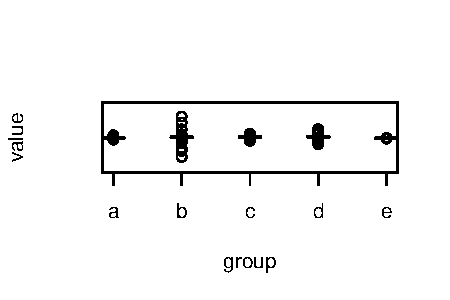
\includegraphics{ex23-1.pdf}
    \end{center}
    



    \begin{center}
\begin{tabular}{rrrrrr}
  \hline
  & a & b & c & d & e \\ 
  \hline
  $n_i$ &  20 & 21 & 14 & 11 & 14 \\
  $\bar y_i$ & 1.9985894 & 0.4176685 & 0.9994830 & -0.6623678 & 2.7572143 \\
  $s_i$ & 3.9715284 & 11.1465035 & 0.8638515 & 8.3122179 & 3.9775048 \\
   \hline
\end{tabular}
    \end{center}
\end{frame}

\section{Two-way ANOVA}


%%%%%%
\begin{frame}{``Factorial'' design}

    Often experiments want to examine the combined effects \\
    of several \alert{factors} \\
    in all their possible combinations. \\

    \vspace{2em}

    How does each factor affect the outcome? \\
    Does the \alert{effect} of one factor depend on the other factor?

    \vspace{2em}


    \structure{Examples:}
    \begin{itemize}
        \item (blood pressure) :  (blood pressure medication) $\times$ (age)
          \pause
        \item (beak size) : (sex) $\times$ (island)
          \pause
        \item (plant growth rate) : (water) $\times$ (sunlight)
    \end{itemize}


\end{frame}

%%%%%%
\begin{frame}{Example: beak size}

    Beak size of finches in different islands: 
    \vspace{2em}

    (equal sample sizes : a \structure{balanced} design)
    \vspace{2em}

    { \tiny
\begin{tabular}{c|cccccccccc}
    &   a & a & b & b & c & c & d & d & e & e \\
    &   F & M & F & M & F & M & F & M & F & M \\
    \hline
    & 10.89 & 8.62 & 7.32 & 8.13 & 9.99 & 8.14 & 19.13 & 18.34 & 5.73 & 5.48 \\ 
    & 10.44 & 9.13 & 9.77 & 7.87 & 9.73 & 8.30 & 18.50 & 17.57 & 5.89 & 6.61 \\ 
    & 8.49 & 10.21 & 10.16 & 7.74 & 9.41 & 7.80 & 20.72 & 17.60 & 7.93 & 5.08 \\ 
    & 10.60 & 9.36 & 8.97 & 8.61 & 8.71 & 7.08 & 20.21 & 16.72 & 8.34 & 4.93 \\ 
    & 10.72 & 8.47 & 10.20 & 7.88 & 9.05 & 9.50 & 17.65 & 17.63 & 6.56 & 5.55 \\ 
    & 11.41 & 9.09 & 8.12 & 7.67 & 7.43 & 7.96 & 19.54 & 18.26 & 8.03 & 6.97 \\ 
    & 11.19 & 9.27 & 9.26 & 7.27 & 8.39 & 8.67 & 20.04 & 18.34 & 6.78 & 6.74 \\ 
   \hline
$n_i$  &  8     &  8     &  8     &  8      &  8      &  8      &  8     &  8     &  8      &  8      \\
  mean & 10.23 & 9.33 & 9.02 & 7.90 & 8.90 & 8.17 & 19.46 & 17.92 & 7.04 & 6.30 \\ 
  SD   & 1.24 & 0.71 & 1.03 & 0.39 & 0.83 & 0.70 & 1.00 & 0.67 & 0.99 & 1.36 \\ 
\end{tabular}
}
\end{frame}

%%%%%%
\begin{frame}{Example: beak size}

  \alert{Questions:} \\
    \vspace{1em}
    Does mean beak size differ between islands? \\
    \vspace{1em}
    Between sexes?  \\
    \vspace{1em}
    Is the size of the sex difference larger in some islands than others?


    \vspace{2em}

    \only<1>{
  Means, summarized:
\begin{center}
  \begin{tabular}{c|ccccc|c}
    means & a & b & c & d & e &  \\
    \hline
  F & 10.23 & 9.02 & 8.90 & 19.46 & 7.04 & 10.93 \\ 
M & 9.33 & 7.90 & 8.17 & 17.92 & 6.30 & 9.92 \\ 
  \hline
  & 9.78 & 8.46 & 8.54 & 18.69 & 6.67 & 10.43 \\ 
  \end{tabular}
\end{center}
}

    \only<2>{
  Means, relative to grand mean:
\begin{center}
  \begin{tabular}{c|ccccc|c}
    means & a & b & c & d & e &  \\
    \hline
  F & -0.20 & -1.41 & -1.53 & 9.03 & -3.38 & 0.50 \\ 
  M & -1.09 & -2.53 & -2.25 & 7.49 & -4.12 & -0.50 \\ 
  \hline
  & -0.65 & -1.97 & -1.89 & 8.26 & -3.75 & \alert{10.43} \\ 
  \end{tabular}
\end{center}
}

    \only<3>{
  Means, relative to sex and island means:
\begin{center}
  \begin{tabular}{c|ccccc|c}
    means & a & b & c & d & e &  \\
    \hline
    F & -0.06 & 0.06 & -0.14 & 0.27 & -0.13 & \alert{0.50} \\ 
    M & 0.06 & -0.06 & 0.14 & -0.27 & 0.13 & \alert{-0.50} \\ 
    \hline
 & \alert{-0.64} & \alert{-1.96} & \alert{-1.89} & \alert{8.26} & \alert{-3.75} & \alert{10.43} \\
  \end{tabular}
\end{center}
}

\end{frame}

%%%%%%
\begin{frame}{Example: beak size}
    Beak size of finches in different islands\\
    \alert{
    \only<2>{with male/female means subtracted off:}
    \only<3>{with island means subtracted off:}
    \only<4>{with both subtracted off:}
    }
    \begin{center}
        \includegraphics<1>{ex23-beaks.pdf}
        \includegraphics<2>{ex23-beaks-nosex.pdf}
        \includegraphics<3>{ex23-beaks-noisland.pdf}
        \includegraphics<4>{ex23-beaks-nosex-noisland.pdf}
    \end{center}
\end{frame}


%%%%%%
\begin{frame}{Two-way ANOVA model}

  Now, $y_{ijk}$ is the $k^\mathrm{th}$ observation
  in the $i^\mathrm{th}$ group of the first factor
  and the $j^\mathrm{th}$ group of the second factor,
    \[
    y_{ijk} = \mu + \tau_i + \beta_j + \only<2->{\eta_{ij} +} \epsilon_{ijk} ,
    \]
    where \alert{$\mu$} is the population mean, \\
    \alert{$\tau_i$} and \alert{$\beta_j$} are the mean effects of groups $i$ and $j$,\\
    and the \alert{$\epsilon_{ijk}$} are independent noise terms.


    \vspace{2em}
    \pause

    and with \structure{interaction effects}, \\
    \alert{$\eta_{ij}$} is the mean effect of the combination of $i$ and $j$, \\
    after accounting for each group's effect.


\end{frame}

%%%%%%
\begin{frame}{Sum of Squares in Two-way ANOVA}

  Define the residual sample means as before:
    \[
    y_{ijk} = \hat \mu + \hat \tau_i + \hat \beta_j + \hat \eta_{ij} + \hat \epsilon_{ijk} ,
    \]
    and $n_{ij}$ the number of observations in $(i,j)$; 
    $n_{i\cdot} = \sum_j n_{ij}$, and 
    $n_{\cdot j} = \sum_i n_{ij}$.
    \structure{If all the $n_{ij}$ are the same} (``balanced''),\\
    we can still partition the sum of squares:
  \begin{align*}
    \SS(\text{between $i$}) &= \sum_{i} n_{i\cdot} \hat \tau_{i}^2 & \df(\text{between $i$}) &= I-1 \\
    \SS(\text{between $j$}) &= \sum_{j} n_{\cdot j} \hat \beta_{j}^2 & \df(\text{between $j$}) &= J-1 \\
    \SS(\text{interactions}) &= \sum_{ij} n_{ij} \hat \eta_{ij}^2  & \df(\text{interactions}) &= (I-1)(J-1) \\
    \SS(\text{within}) &= \sum_{ijk} \hat \epsilon_{ijk}^2  & \df(\text{within}) &= n_{\cdot} - IJ\\
    \SS(\text{total}) &= \sum_{ijk} (y_{ijk}-\hat \mu)^2 & \df(\text{total}) &= n_\cdot - 1  
  \end{align*}

\end{frame}

%%%%%%
\begin{frame}{$F$-test for two-way ANOVA}

  \structure{General Principle of the $F$ test:}
  \[
  F_s = \frac{ \MS(\text{effect you are testing}) }{ \MS(\text{within}) } 
  \]

    \vspace{2em}

    \structure{Why?} $\MS(\text{within})$ estimates the within-group SD.

\end{frame}

%%%%%%
\begin{frame}{$F$-tests, beak sizes:}

    \[
    y_{\text{island},\text{sex},k} =  \mu +  \tau_\text{island} +  \beta_\text{sex} +  \eta_{\text{island},\text{sex}} +  \epsilon_{\text{island},\text{sex},k} 
    \]


    \only<1>{
    Are there \alert{sex differences} in mean beak size that are of \structure{different sizes on different islands}?
  (or, Are mean beak size effects of sex and island \emph{not} additive?)
  \begin{align*} 
    H_0 &: \quad \eta_{11} = \eta_{12} = \cdots = \eta_{I-1,J} = \eta_{IJ} = 0 \\
    F_s &= \frac{ \MS(\text{interaction}) }{ \MS(\text{within}) } = \frac{0.776}{1.060} = 0.7318\\
    df &= (4,70)
  \end{align*} 
  }
  

  \only<2>{
  Are there differences in mean beak size \structure{between islands} (consistent across both sexes)?
  \begin{align*} 
    H_0 &: \quad \tau_1 = \cdots = \tau_I = 0 \\
    F_s &= \frac{ \MS(\text{between islands}) }{ \MS(\text{within}) } = \frac{43.478}{1.060} = 41.0228 \\
    df &= (4,70)
  \end{align*} 
  }

  \only<3>{
  Are there differences in mean beak size \structure{between sexes} (consistent across all islands)?
  \begin{align*} 
    H_0 &: \quad \beta_1 = \cdots = \beta_J = 0 \\
    F_s &= \frac{ \MS(\text{between sexes}) }{ \MS(\text{within}) } = \frac{23.032}{1.060} = 21.7317 \\
    df &= (1,70)
  \end{align*} 
  }


\end{frame}

%%%%%%
\begin{frame}{$F$-tests, summary:}

  \begin{center}
    \begin{tabular}{c|ccccc}
 & df & Sum Sq & Mean Sq & F value & $P$  \\
 \hline
island & 4 & 173.912 & 43.478 & 41.0228 & $<$.000001 \\
sex & 1 & 23.032 & 23.032 & 21.7317 & .000014 \\
interaction & 4 & 3.102 & 0.776 & 0.7318 & 0.5733  \\
within & 70 & 74.189 & 1.060 &  & \\
\hline
total & 79 & 274.235 & & & \\
\end{tabular}
\end{center}


    \vspace{2em}

    \structure{Conclusion:} We have very strong evidence that mean beak size varies between sexes, and by island, but have no evidence that these effects are not additive.

\end{frame}



\section<article>{Summary}
\section<presentation>*{Summary}

\begin{frame}{Summary}
  \begin{enumerate}
    \item The $F$ test is the ratio of mean squares, between to within,
    \item and tests for significant differences between group means.
    \item To be sensible, it needs independent samples and similar within-group SDs.
    \item The ANOVA framework extends to multifactorial designs,
    \item but follows the same principle of comparing means squares between to within.
  \end{enumerate}
\end{frame}

% homework
\begin{frame}{Homework}
  \begin{center}

  11.4.5

  \vspace{2em}


  11.7.1

  \vspace{2em}

  11.7.2

  \end{center}
\end{frame}


\end{document}





Or, Sticklebacks (has plot): http://www.plosone.org/article/info%3Adoi%2F10.1371%2Fjournal.pone.0059644

From http://www.sciencemag.org.libproxy.usc.edu/content/296/5568/707.full:

The first samples in 1973 (221 G. fortis and 72 G. scandens) were compared by ANOVAs with the last samples in 2001 (114 G. fortis and 35 G. scandens). The data were trimmed to 2.5 SD on either side of the mean by removing one to three individuals from the samples of each species. This corrected for skewness and unequal variances. Sex was included in two-factor ANOVAs because males are generally larger than females. Mean body size was significantly smaller in G. fortis (F 1,132 = 7.773, P = 0.0061) and in G. scandens (F 1,50 = 11.272, P < 0.0001) in 2001 than in 1973. There was a significant effect of sex in each species (P < 0.002) but no sex-by-year interaction (P > 0.1). Mean beak size did not differ between years in either G. fortis (F 1,166 = 0.004, P = 0.9480) or G. scandens (F 1,50 = 3.108, P= 0.0840); sex effects were significant in both species (P< 0.007), but there were no sex-by-year interactions (P> 0.1). Beak shape differed between years in both species. For G. scandens there was a strong year effect (F 1,72 = 17.168, P < 0.0001), a weak sex effect (F 1,72 = 5.943, P = 0.0172), and no interaction. The G. fortis sexes do not differ in beak shape (P = 0.9715), and therefore a one-factor ANOVA was performed with adult males, females, and birds of unknown sex. It demonstrated a strong difference between years (F 1,287 = 30.246, P < 0.0001). 

